\section{Research Methodology}
The quality of any project is governed by three key factors: cost, time, and scope, all of which must be managed efficiently throughout the project's lifetime. As a result, methodologies are required. Saunders  Research Onion Model \autocite{saunders2003research} has been used to deduce the methodologies. 
The methodologies chosen as appropriate for the project are listed in the table below.

\begin{longtable}{| p{0.11\linewidth} | p{0.88\linewidth}|}
\caption{Research Methodology}
\label{tab:research-methodology-table}\\
\hline
Research Philosophy  & The philosophy of research influences data collection \& data analysis since it is related to the nature of reality being investigated.

Positivism, Interpretivism \& Constructivism are philosophies that could be used to approach this research. Out of these, \textbf{Positivism} was chosen since the research is expected to be replicable with similar \textbf{quantifiable} results.
\\
\hline
Research Approach & The approach that a researcher may use when conducting the research is the approach.

A \textbf{Deductive} approach was chosen over an Inductive approach since this is expected to be a \textbf{quantitative} research that aims to \textbf{test \& prove} the \textbf{hypothesis} at hand. \\
\hline
Research Strategy  &The strategy focuses on the data collection methods that will be used to answer the research questions.

\textbf{Survey, Archival Research} \& \textbf{Ethnography} were the strategies chosen to address the research questions. These strategies were chosen as they would compliment each other while providing relevant data that is enough for the research. While Survey seems to be the primary strategy, Archival Research \& Ethnography is expected to allow the qualitative aspect expected in the approach taken to the solution, which will finally affect the \textbf{quantitative results}, to be addressed. \\
\hline
Research Choice & Choice of the methodology identifies if the research is concerned with the qualitative and quantitative aspects of the research.


\textbf{Multi-method} was chosen since although \textbf{quantitative results} are the primary  perspective, it is identified that qualitativeness of the data used by the system to be developed will also be an important consideration that will affect the quantitative results.\\
\hline
Time Horizons  & 

\textbf{Longitudinal} was chosen as the time horizon for the research since data will be gathered and used for evaluation and testing over a long period of time.\\
\hline
Techniques and procedures &  Data collection and analysis techniques are considered here.

Mediums such as online news, statistics \& trends from social media, observations, conversations, reports, surveys, documents, secondary tabular data, organizational records will be used.\\
\hline
\end{longtable}


\section{Development Methodology}
\subsection{Life cycle model}
\textbf{Agile} Software Development Life-cycle was chosen as the research development method since iterative development is needed.

\subsection{Design Methodology}
% Design Paradigm
% SSADM or OOAD or Anything else?
Object-Oriented Analysis and Design were chosen as the Design Methodology by the author to support an incremental methodology that can be used to extend the system with the ability to reuse system components.

\subsection{Evaluation Methodology}
As identified in recent advancements in literature \autocite{larry_history_2019}, \gls{p@k} score has been identified as a suitable method of evaluating a Recommendations System. This is also identified as the Top-N strategy in several past literatures. Therefore, it will be used to compare the novel solution that is to be developed against baseline models.

\subsubsection{Benchmarking}
Precision, recall, \gls{mae} and \gls{rmse} will be used to Benchmark the Recommendation System \autocite{dayan_recommenders_2011}, to help evaluate future researches in this domain by conducting comparative benchmarking-analysis.


\section{Project Management Methodology}
\textbf{Prince2}  was chosen as the project management methodology. It allows the author to develop the product in controlled environments in logical compartmentalized units.
 
\newpage
\subsection{Schedule}
\subsubsection{Gantt Chart}
% Gantt Chart
\begin{figure}[h!]
\centering
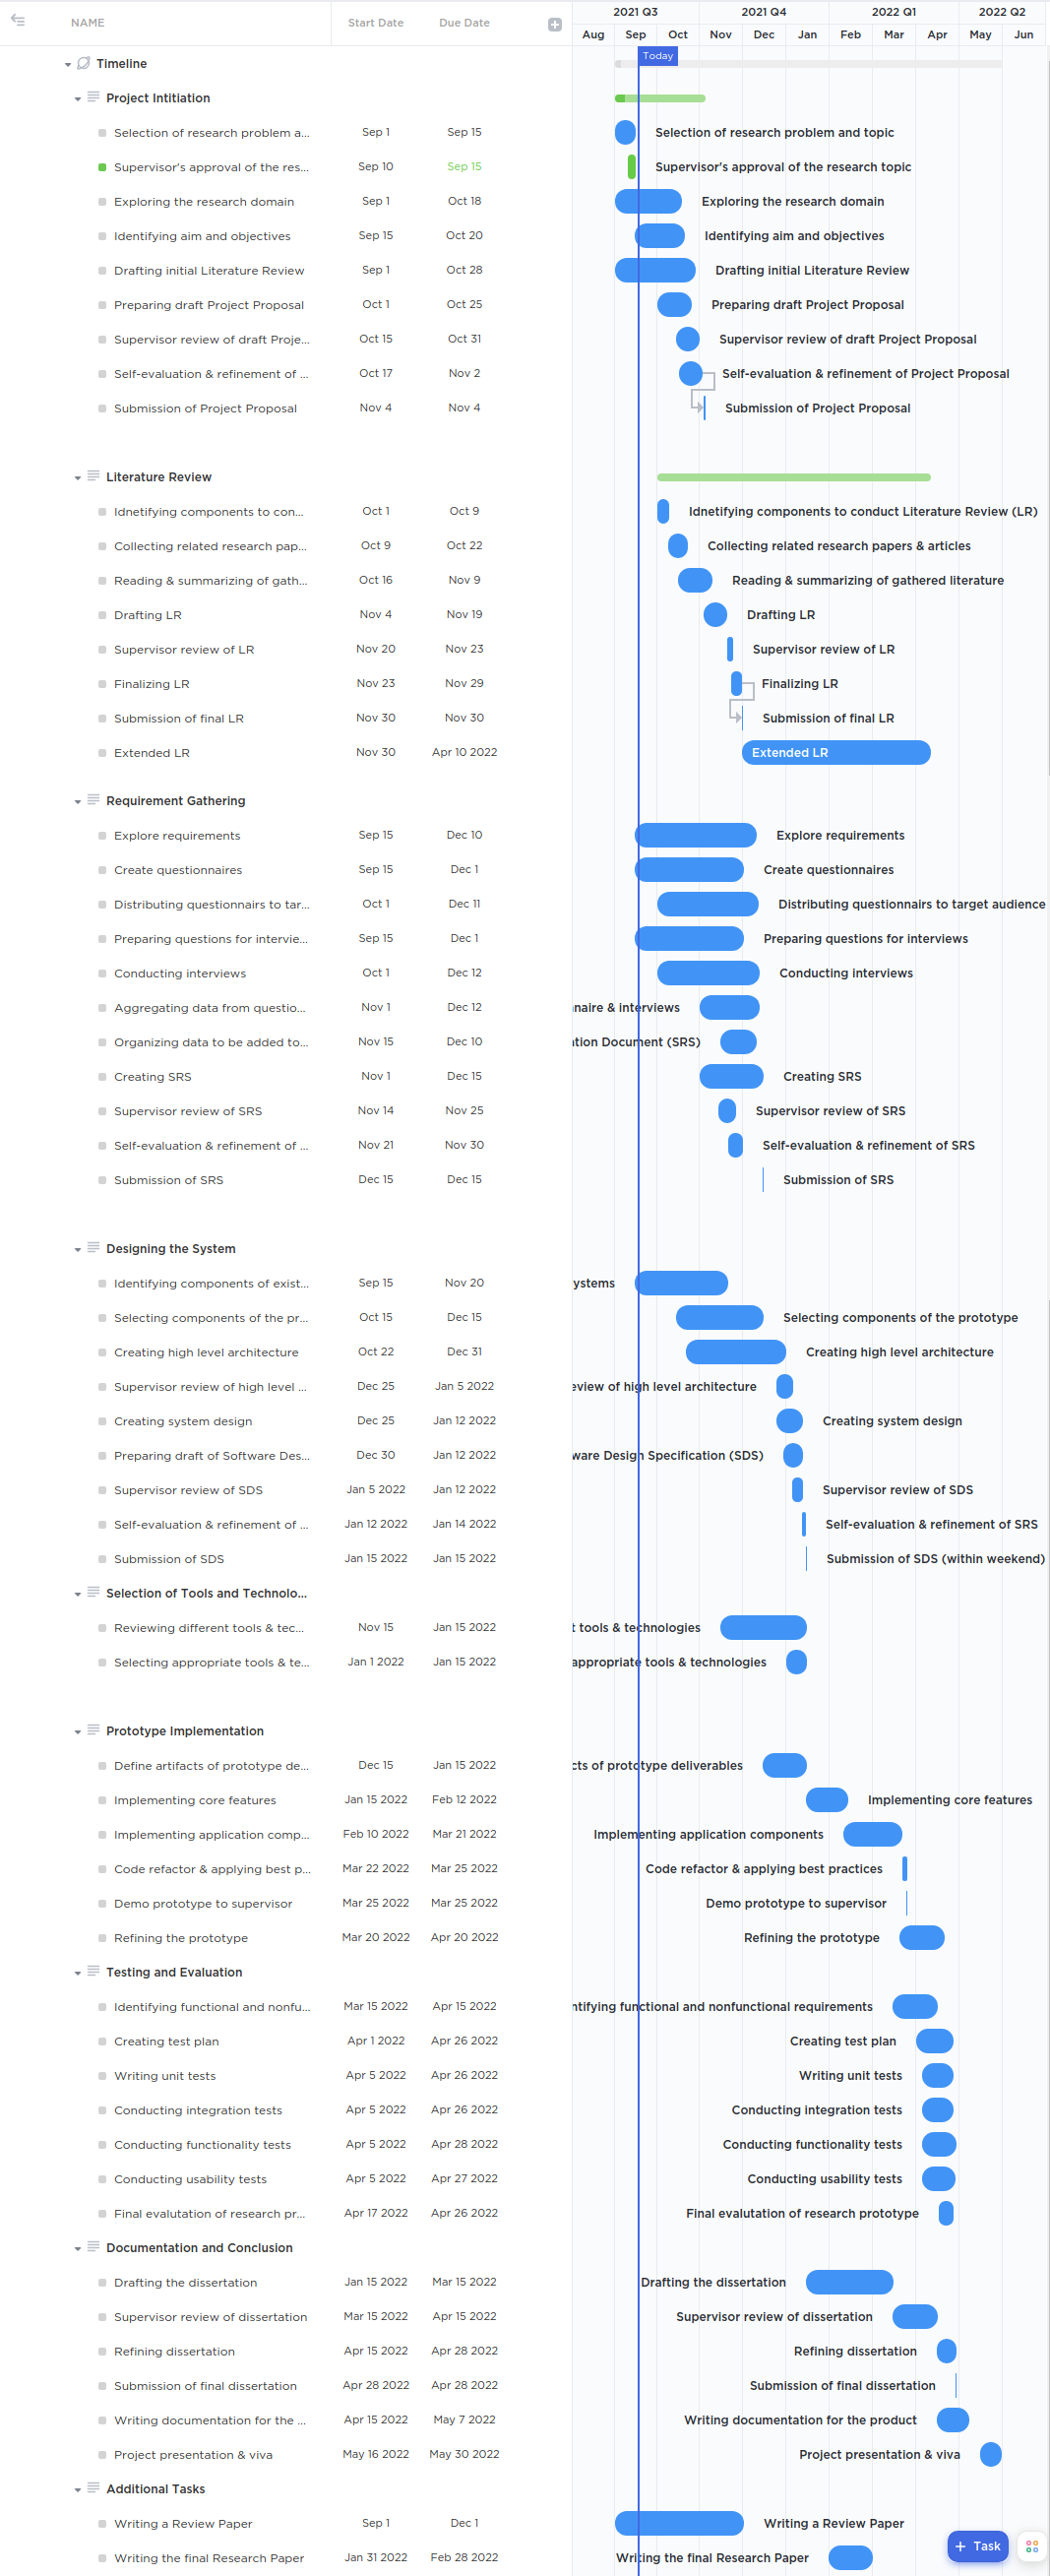
\includegraphics[width=0.8\textwidth,height=0.85\textheight]{images/gantt-chart.png}
\caption{Gantt Chart}
\end{figure}


\newpage
\subsubsection{Deliverables}
\vspace{-7mm}       % remove spacing

% \centering
\begin{longtable}{| p{0.76\linewidth} | p{0.22\linewidth}|}
\caption{Deliverables and dates}
\label{tab:deliverables-table}\\
\hline
Deliverable &   Date  \\ 
\hline
\textbf{Project Proposal Document}    &   4\textsuperscript{th} November 2021\\
% \cline{1-1}
The initial proposal of the project  &  \\ 
\hline
\textbf{Literature Review Document} & 11\textsuperscript{th}~December 2021  \\ 
The Critical review of existing work and solutions  & \\ 
\hline
\textbf{Software Requirement Specification} & 15\textsuperscript{th}~December 2021 \\ 
The document specifying requirements to be satisfied and developed as the final prototype and means of collecting data &    \\ 
\hline
\textbf{System Design Document} & 1\textsuperscript{st}~December 2021  \\ 
The document specifying the design developed for the Recommendations System and overviews of the algorithms to be developed.    &   \\ 
\hline
\textbf{Prototype}  & 1\textsuperscript{st}~February 2022   \\
The prototype with main core features functional    &    \\ \hline
\textbf{Thesis} & 15\textsuperscript{th}~March 2022  \\  The final report documenting the project and research process and decisions          &   \\ 
\hline
\textbf{Review Paper}  &  1\textsuperscript{st}~March 2022     \\ 
A review paper reviewing existing systems in the Recommendations domain published in a journal/ conference    &   \\ 
\hline
% \textbf{Manuscript Paper}   &  31\textsuperscript{st}~December 2021 \\ 
% A research paper introducing the concepts and design developed as part of this project &   \\ 
% \hline
\textbf{Final Research Paper}   &   1\textsuperscript{st}~April 2021    \\ 
A research paper introducing the Recommendations System developed at the end of this project    &    \\ 
\hline
\textbf{Public project library}   &   1\textsuperscript{st}~April 2021 \\ 
A publicly accessible project library/ repository to set up, test and use the developed Recommendations System  &   \\
\hline
\end{longtable}

\subsection{Resource Requirements}
The resources required to complete the project are identified based on the objectives, expected solutions, and deliverables. The following are the software, hardware, and data resource requirements.

\subsubsection{Software Requirements}
\begin{itemize}
\item \textbf{Operating System(Linux/ macOS/ Windows)} - Linux will be the default choice for development since of the ease of support for multiple development tools and performance benefits. macOS/ Windows will be used for research documentation \& study purposes.
\item \textbf{Python} - The language that will be used to create the Machine Learning \& Deep Learning models. Python is an all-purpose language that has been used in many projects that integrate with data science.
\item \textbf{Tensorflow/ Scikit learn Python packages} - Libraries that will be used to support model development, training \& testing.
\item \textbf{Golang/ NodeJS} - The API that will be used to communicate with the \Gls{ml} backend and the front-end. Golang will allow the application to support concurrency and multi-threaded communications while being extremely lightweight and fast. This will be used to avoid any bottlenecks that could occur at this point in the system. NodeJS will be kept as a secondary option in the case of requiring any pre-built features that are not directly supported by Golang \& aren't directly relevant to the research.
\item \textbf{JavaScript (React)} - The front-end of the application, where recommendations will be shown. This is also an important part of the project since it will be the users' point of interaction with the system.
\item \textbf{PyCharm/ VSCode/ GoLand} - Development environments to support development of the project.
\item \textbf{Google Colab} - Cloud development environment to build, train \& test ML \& Deep Learning models.
\item \textbf{Zotero} - Research management tool to save and backup research artifacts \& manage references.
\item \textbf{Overleaf/ MS Office/ Google Docs/ Canva/ Figma} - Tools to create reports, figures \& documentations.
\item \textbf{Google Drive/ GitHub} - To backup files \& code related to the project
\item \textbf{Docker} - To make the ensemble system's setup process as simple as possible.
\end{itemize}

\subsubsection{Hardware Requirements}
\begin{itemize}
\item \textbf{Core i7x Processor(8\textsuperscript{th} generation) or above} - To be able to perform high resource intensive tasks.
\item \textbf{Nvidia 1050Ti GPU or above} - To manage training processes of data science models.
\item \textbf{16GB RAM or above} - To manage data-sets \& development environments.
\item \textbf{Disk space of 40GB or above} - To store data \& application code.
\end{itemize}

\subsubsection{Data Requirements}
\begin{itemize}
\item \textbf{Non-fungible Token data} - From OpenSea open-API.
\item \textbf{Twitter data} - From Twitter developer API.
\item \textbf{Google Trends data} - From Google Dataset Search \& unofficial Google Trends Python API (Pytrends).
\item \textbf{Ethereum Smart Contract data} - From Etherscan
\item \textbf{User Preference Profiles data} - From Amazon, Yelp, Kaggle open datasets. May be needed for testing purposes.
\end{itemize}

\subsubsection{Skill Requirements}
\begin{itemize}
\item Creation of required Recommendation Systems.
\item Ability to create optimized Machine Learning \& Deep Learning models.
\item Research writing skills.
\end{itemize}

\subsection{Risk Management}
The following are the risks identified prior to starting the project with possible mitigation steps.

\begin{longtable}{| p{0.33\linewidth} |p{0.11\linewidth}| p{0.11\linewidth}| p{0.34\linewidth}|}
\caption{Risk Mitigation Plan}
\label{tab:risk-mitigation-table}\\
\hline
Risk Item & Severity & Frequency & Mitigation Plan \\
\hline
Loose access to on going development code & 5 & 2 & Keep all code backed up on GitHub \& external backup \\
\hline
Corruption of documentation & 4 & 4 & Follow a cloud-first documentation approach and backup on a weekly basis \\
\hline
Inability to complete all expected deliverables within the allocated time & 4 & 2 & Work on deliverables on a priority basis. \\
\hline
Inability to explain the research work done due to illness & 2 & 1 & Have a recording of demonstration and detailed documentation with explanation \\
\hline
\end{longtable}

\subsection{Chapter Summary}